
\section{Jaco-Arm}

\begin{frame}[b]
	\begin{figure}
		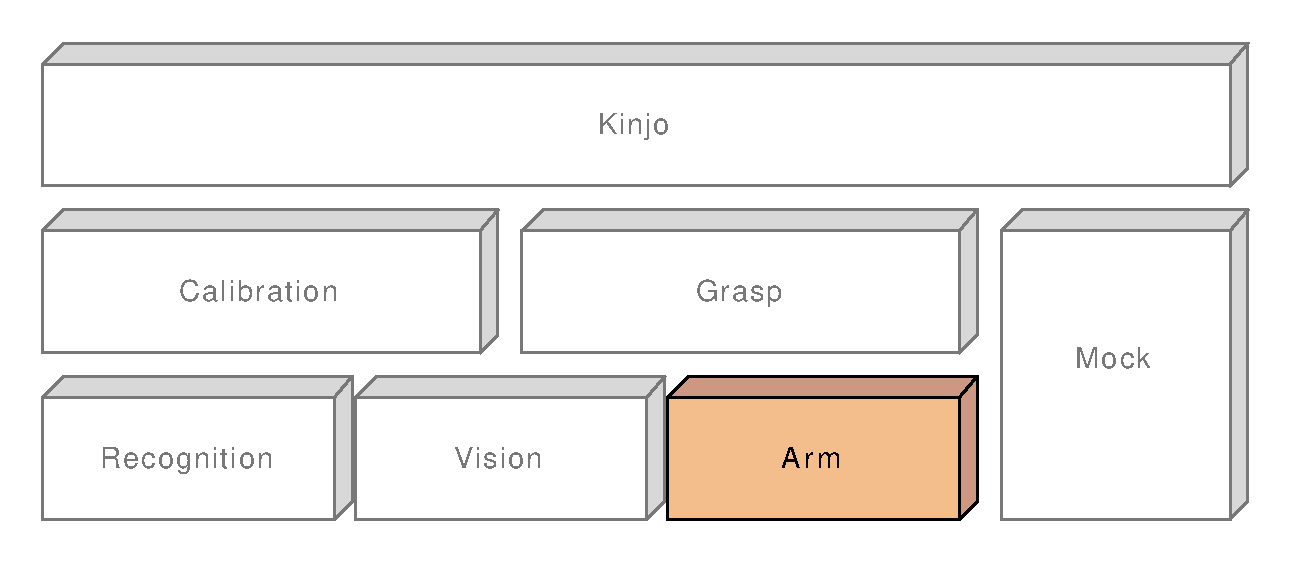
\includegraphics[width=0.8\textwidth]{nav_arm}
	\end{figure}
	\vspace*{0.7cm}
\end{frame}

\begin{frame}[t]{Jaco-Arm}
	\begin{block}{Koordinatensystem}
		\begin{itemize}
			\item Koordinatenursprung etwa Höhe des ersten Aktors
			\item Endeffektor zwischen Fingerspitzen
			\item Treiber liefert Angaben in Metern
		\end{itemize}
		\begin{figure}
			\includegraphics[width=0.5\textwidth]{arm_coordsys}
		\end{figure}
	\end{block}
\end{frame}

\begin{frame}[t]{Jaco-Arm}
	\begin{block}{API}
		\begin{itemize}
			\item Auswahl zwischen C\# (Kinova) und C++ (Fawkes)
			\item Entscheidung für C++ API, da plattformunabhängig
			\item Steuerungsmöglichkeiten:
				\begin{itemize}
					\item Virtueller 6D-Joystick
					\item Absolutes Koordinatensystem
					\item Relative Motorstellung
				\end{itemize}
		\end{itemize}
	\end{block}
\end{frame}

\begin{frame}[t]{Jaco-Arm}
	\begin{block}{Probleme und Lösungen}
		\begin{itemize}
			\item Unmögliche Positionen und Anfahrtswege \arrow Definition von
				\enquote{Deadzones}
			\item Bewegungseinschränkung bei ungünstiger Handausrichtung \arrow
				Startposition mit nach unten gerichteter Hand
			\item Abweichung der Endposition um 4-11mm im virtuellen
				Koordinatensystem \arrow wird z.\,Z. untersucht
			\item Abweichung der Endposition bis zu 8cm im realen
				Koordinatensystem \arrow wird z.\,Z. untersucht
			\item Abdriften beim Rotieren der Hand \arrow Steuerung über virtuellen
				Joystick statt durch absolutes Koordinatensystem
		\end{itemize}
	\end{block}
\end{frame}

\begin{frame}[t]{Jaco-Arm}
	\begin{figure}
		\begin{tabular}{lp{0.5cm}r}
			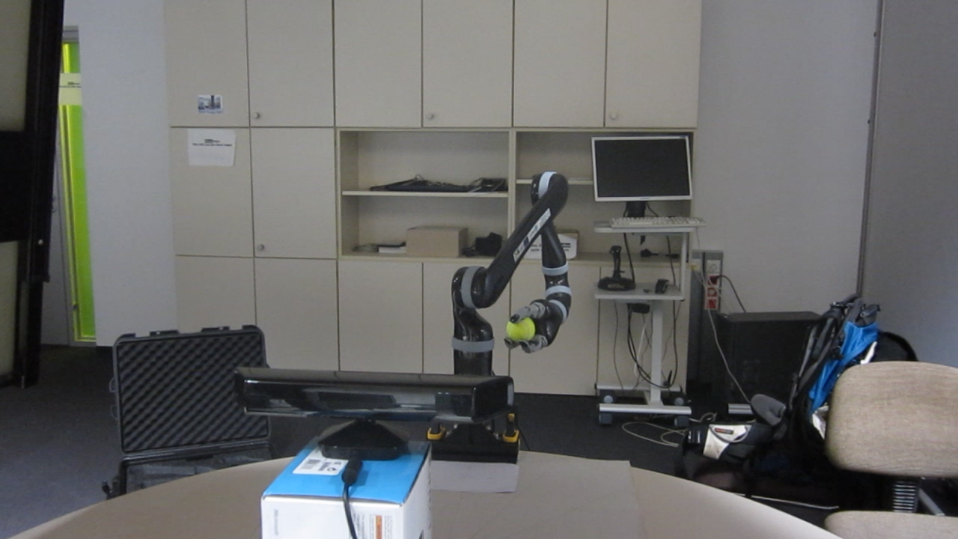
\includegraphics[width=0.3\textwidth, trim=400 100 300 100, clip]{arm_bad} &
			&
			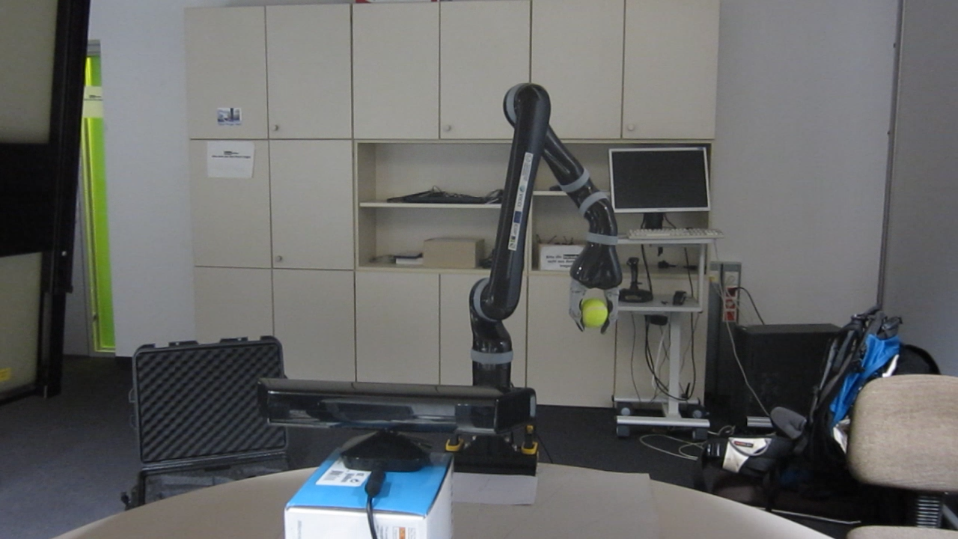
\includegraphics[width=0.3\textwidth, trim=400 100 300 100, clip]{arm_good} \\
		\end{tabular}
		\caption{Bewegungseinschränkende (links) und -begünstigende Handstellung (rechts)}
	\end{figure}
\end{frame}

